\documentclass[12pt]{article}
\usepackage[breaklinks=true]{hyperref}
\usepackage[margin=0.75in]{geometry}

\usepackage{graphicx}
\usepackage{color}

\definecolor{pblue}{rgb}{0.13,0.13,1}
\definecolor{pgreen}{rgb}{0,0.5,0}
\definecolor{pred}{rgb}{0.9,0,0}
\definecolor{pgrey}{rgb}{0.46,0.45,0.48}

\usepackage{listings}
\lstset{language=Java,
  showspaces=false,
  showtabs=false,
  tabsize=2,
  breaklines=true,
  showstringspaces=false,
  breakatwhitespace=true,
  commentstyle=\color{pgreen},
  keywordstyle=\color{pblue},
  stringstyle=\color{pred},
  basicstyle=\ttfamily,
  frame=single,
  moredelim=[il][\textcolor{pgrey}]{$$},
  moredelim=[is][\textcolor{pgrey}]{\%\%}{\%\%}
}

\title{Java Collections}
\author{
	Melvyn Ian Drag
}
\date{\today}


\begin{document}
\maketitle

\begin{abstract}
$java.util$ provides many containers. These containers are widely used in Java programming and are implementations of the great data structures you hear about in data structures \& algorithms classes. In today's lecture we'll have a look at a few of them and consider when we would want to use them.
\end{abstract}

\section{Exam}
Anyone who submitted by now and the code works gets a 100 automatically. Anyone who didn't submit or who submitted something broken can submit by next week for up to 80\% of the grade. These folks will still have to defend their code as described before.

\subsection{How to do the exam}
Take 10 minutes and solve the exam problem in front of students.

\subsection{Historical Pass Rate}
The historical pass rate for this class is 50\%. There are some people saying the class is too hard - but those people are in the bottom 50\% so I statistically that means these people would have not passed even if I made the class easier as it has been in previous semesters.

\section{Introduction}
A java collection is a container you can use to store a bunch of values. For example, in your program you may need to store a bunch of ages - in this case you would

\begin{lstlisting}
...
int[] ageArray = {19, 25, 13, 41, 15};
...
\end{lstlisting} 

or you might create a class called 'Person' and when want to store a bunch of People. In this case you might

\begin{lstlisting}
Person[] peopleArr = { new Person(), new Person(), ...};
\end{lstlisting}

in these two examples I am using arrays. While arrays are fine for simple collections of items, there are some distinct disadvantages of using arrays compared to using a more elegant container. There are some cases where using an array is extremely problematic. One major disadvantage is that the array size is fixed. Once you create an array of 5  elements , you cannot add a sixth person to the array.  

There are many Java Collections. For example, 

\begin{enumerate}
\item ArrayList
\item LinkedList
\item Vector
\item PriorityQueue
\item ArrayDeque
\item HashSet
\item LinkedHashSet
\item TreeSet
\item HashMap
\item TreeMap
\item LinkedHashMap
\item ConcurrentListSkipMap
\item WeakHashMap
\item Stack
\item etc.
\end{enumerate}

We are going to focus on just a few of them today. Namely, we will compare

\begin{enumerate}
\item ArrayList
\item LinkedList
\end{enumerate}

\section{What is a list?}
A list is an abstract idea - it's a bunch of objects in a row, like the arrays that we've seen so far. The list contains a bunch of items. You can delete items from it and add items to it. As I said before - big drawback of arrays is that the size of an array is fixed.

\lstinputlisting{IntArrayCreator.java}

Note that all of the above arrays have four elements in them, and that cannot be changed! Sometimes that's what you want, sometimes thats not. Your call. If you want a variable number of elements in your container, use a List not an array.

\section{What is an ArrayList?}
\subsection{overview}
An ArrayList is a container like an array, but the size isn't fixed. You can put some elements of a specified type in them. See this example to create ArrayLists of different types:

\lstinputlisting{ArrayListDemo.java}

WARNING! This code won't work:
\begin{lstlisting}
...
ArrayList<int> intArrayList = new ArrayList<int>();
...
\end{lstlisting}

because you can't put primitive types in an ArrayList - only reference types ( i.e. everything except primitives )
You can't put any of these in an ArrayList

\begin{itemize}
\item byte
\item float
\item int
\item double
\end{itemize}

but the ``Byte", ``Float", ``Int" and ``Double" types are okay, because these aren't primitives, they are classes.


\section{Exercise: Create 5 different ArrayLists, each holding a different type.}

Allow 10 minutes to ensure that everyone can use the arraylists successfully.


\section{What is a LinkedList?}
To be perfectly honest, I've not yet researched how linked lists are implemented in Java, but I have studied algorithms and I've see how they are implemented in other languages. I'll give you a bit of information now and then we'll do some experiments to see if Java aligns with our expectations.

\textit{Draw a linked list on the board} 

\textit{Read the wikipedia article on linked lists}

I will improvise this section about a linked list. If you don't understand the concept after our discussion in class, you can look on youtube. Sometimes hearing different people say the same things makes those things easier to understand.

\section{The Collections Interface}
Here is a good picture I found to explain the collections interface:

\begin{figure}[h]
  \centering
    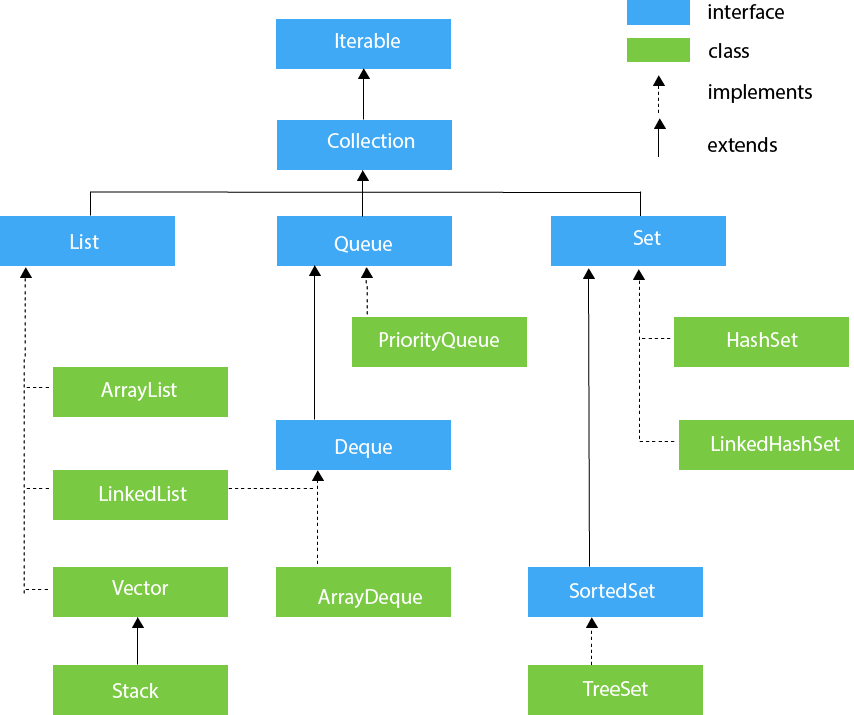
\includegraphics[width=0.5\textwidth]{java-collection-hierarchy.png}
  \caption{Illustration of a variety of classes which implement the Collection class.}
\end{figure}


What are some methods that the  collections interface supplies?

\subsection{Exercise}
I could have written a long lesson on this, but I think it's better that we just find out together. I'm not sure what the collection interface supplies - I could spend an hour now researching and implementing some code, but why don't we do it together?

\subsection{Reference}


\url{https://www.javatpoint.com/collections-in-java}

\section{Initializing a List\textless T\textgreater with an ArrayList\textless T\textgreater or LinkedList\textless T\textgreater}
Weird thing that Java programmers do. Java programmers use this pattern to achieve a bunch of complex things that you won't learn about in this class. Grab a good book and learn to write a Java Web App or Android App and you will see this pattern used in certain ways to achieve particular ends.

\begin{lstlisting}
List<String> l = new ArrayList<String>(){"Hello", "World"};
\end{lstlisting}

\section{Timing Comparison}
In this section we'll measure how long different datastructures take to perform different tasks. The reason different data structures exist is that they have different strengths and weaknesses, and programmers might need a datastructure that performs well in a certain situation. This talk is somewhat abstract if you haven't taken  a data structures and algorithms class. There you learn things like ``Computational Complexity" and ``Big O" notation. We're only going to focus now on the simplest of examples to give you a taste of whats to come ( for those who haven't yet studied data structures). For those who already know about datastructures, I'm hoping you're still interested in discussing them.

\subsection{How To Time Code}
There are many ways to measure time with Java. I'll just show you one. Java knows how many milliseconds have passed since the \textbf{Epoch}. When is the Epoch? Why is it important I can't remember, but it is a commonly used "t0" in computer science, especially on unix systems. 



2. Compare the following operations:

Do the add and remove operations. Discuss the complexity of those operations, and then work it out in class.



\section{Why Are Collections Useful?}
In case I haven't made it abundantly clear through examples by now, collections are very useful and interesting. Here is the official pitch from Oracle about why Java collections are useful:
\url{file:///home/melvyn/Desktop/JavaFall2019ClassRepo/ReadingMaterials/tutorial/collections/intro/index.html}

\subsection{highlight these points}
\begin{itemize}
\item reduces effort - you never need to code up a dynamically resizing array, because Java has one, for example
\item increases quality - for example, the linked list implementation you are likely to write will be buggy and slow. The one in the collections framework has been tweaked and perfected by experts for a long time.
\item Interoperability between different APIS - since we all agree to use standard collections, all our code can interact. If everyone used a different linked list implementation you couldn't pass data between different peoples' codes.
\end{itemize}

BTW If you don't know what an \textbf{API} is, it means \textbf{Application Programming Interface}. It pretty much means the publicly facing part of your code that other people can access. That may not be helpful - an example is warranted here.

There is a good chance that you know next to nothing about linked lists outside of what I've told you today. Even if you have studied algorithms and data structures, you probably implemented a very simplistic linked list. Nevertheless, today you learned how to add, and remove elements from a linked list. That is because it has a good API. You, the \textbf{Application Programmer}, only have to know a few functions, you don't need to understand the guts of the whole linked list code to use it. The API is the set of publicly accessible functions that application programmers will use.
\end{document}
